\chapter{假设检验}

\section{假设检验的概念}

\subsection{基本思想}

\textbf{基本思想}:将参数空间$\Theta$拆分为两个不相交的集合$\Theta_0, \Theta_A$即
\[ \Theta_0 \cap \Theta_A=\emptyset,\ \Theta_0 \cup \Theta_A=\Theta \]
接下来通过数据选择应该接受两个假设
\[ H_0:\Theta \in \Theta_0,\ H_A:\Theta \in \Theta_A \]
中的哪一个。

\textbf{问}:是否能用点估计代替假设检验?即若估计结果$\hat{\theta} \in \Theta_0$,则接受假设$H_0$;或反之。

假设某一总体遵循二项分布$B(n,p)$,做出如下假设:
\[ H_0:p=0.5,\ H_A : p \neq 0.5 \]
若$n=10^5$,估计值$\hat{p}=0.50001$。按估计结果应认为$H_A$成立,然而一般按情理而言,似乎$H_0$更恰当。这体现出点估计与假设检验的不同:点估计的结果是客观的;而假设检验的结果包含一定的主观性。

若假设可用一个参数的集合表示,该假设检验问题称为\textbf{参数假设检验}问题,否则称为\textbf{非参数假设检验}问题。上例就是一个参数假设检验问题,而对假设“总体为正态分布”作出检验的问题则是一个非参数假设检验问题。

\begin{definition}[原假设与对立假设]
    设有来自某一个参数分布族$\{ F(x,\theta) | \theta \in \Theta \}$的样本$x_1,\cdots ,x_n$,其中$\Theta$为参数空间。设$\Theta_0 \in \Theta,\ \Theta_0 \neq \emptyset$,则命题$ H_0:\theta \in \Theta_0$称为或\textbf{原假设}或零假设(null hypothesis);并称命题$H_A:\theta \in \Theta_A,\ \Theta_A=\Theta-\Theta_0$为$H_0$的\textbf{对立假设}或备择假设(alternative hypothesis)。
\end{definition}
\begin{remark}
    原假设与对立假设之间是否不同呢?可以任意交换吗?答案参见\ref{subsec:neyman-pearson-paradigm}节
\end{remark}

\begin{definition}
    如果假设(原假设或对立假设)只含一个分布,则称之为\textbf{简单假设}(simple hypothesis),否则称为\textbf{复合假设}(composite hypothesis)。
\end{definition}

\begin{example}[硬币辨别实验]\label{ex:coins}
    问题情景:假设有两个硬币,其中一个丢出正面的概率为$0.7$,另一个为$0.5$。现在随机取出其中一个硬币,丢了$10$次,并且记录下出现正面的次数$X$。根据这些数据,如何决定取出的时哪个硬币?

    统计模型:
    \begin{itemize}
        \item $X \sim \Binomial(10,p)$
        \item $\Theta = \{p: 0.5, 0.7 \}$
    \end{itemize}

    数学描述:
    \begin{itemize}
        \item $H_0: p=0.5$,即 $\Theta_0=\{ 0.5 \}$
        \item $H_A: p=0.7$,即 $\Theta_A=\{ 0.7 \}$
    \end{itemize}
    皆为简单假设。
\end{example}

当$H_0$为简单假设时,其形式可写成$H_0:\theta = \theta_0$,此时的备择假设通常有如下三种可能:
\[ H_A':\theta \neq \theta_0,\ H_A'':\theta < \theta_0,\ H_A''':\theta > \theta_0,\ \]
称$H_0 \vs H_A'$为双侧假设或\textbf{双边假设};$H_0 \vs H_A''$以及$H_0 \vs H_A'''$为单侧假设或\textbf{单边假设}。

\begin{example}[超能力检验]
    问题情景:现在从一副扑克牌中随机抽出一张牌,让被检验者猜测牌的花色,有放回地重复20次,记下猜对的次数T。根据这些数据,如何判断被检验者是否有超能力?

    统计模型:假设被检验者猜对的概率为$p$。
    \begin{itemize}
        \item $T \sim \Binomial(20,p)$
        \item $\Theta = \{p: p \in [0.25,1]\}$(代表被检验者的能力总比完全瞎蒙强),或者$\Theta = \{p: p \in [0,1]\}$(有可能比完全瞎蒙弱)
    \end{itemize}

    数学描述:
    \begin{itemize}
        \item 若$\Theta = \{p: p \in [0.25,1]\}$,则
              \[ H_0: p=0.25 \vs H_A: p > 0.25  \]
              即$\Theta_0=\{ 0.25 \},\ \Theta_A=(0.25,1]$。$H_0$为简单假设,$H_A$为复杂假设,也为单边假设。
        \item 若$\Theta = \{p: p \in [0,1]\}$,则
              \[ H_0: p=0.25 \vs H_A: p \neq 0.25  \]
              即$\Theta_0=\{ 0.25 \},\ \Theta_A=[0,0.25)\cup (0.25,1]$。$H_0,H_A$都是复杂假设,$H_A$为双边假设。
    \end{itemize}
\end{example}

\begin{example}[拟合优度检验]
    问题情景:假设有$n$个样本 $X_1,\cdots ,X_n$,已知他们独立同分布,并来自于一个离散总体,如何判断它们来自Poisson分布?

    统计模型:
    \begin{itemize}
        \item $X_1,\cdots ,X_n \overset{\text{i.i.d.}}{\sim} F$
        \item $\Theta = \{F: F\text{是离散分布} \}$
    \end{itemize}

    数学描述:
    \begin{itemize}
        \item $H_0: \text{来自Poisson分布}$,即 $\Theta_0=\{\Poisson(\lambda),\ \lambda>0   \}$
        \item $H_A: \text{不来自Poisson分布}$,即 $\Theta_A=\Theta \setminus \Theta_0$
    \end{itemize}
    皆为复杂假设。
\end{example}

\subsection{Neyman-Pearson范式}\label{subsec:neyman-pearson-paradigm}

\begin{definition}
    对于样本空间$S$,若有一种规则将其划分为两个互不相交的区域$K,K^{\complement}$,并且当样本$x \in W$时,选择假设$H_A$,否则接受假设$H_0$,则将这种划分称为\textbf{检定}(test),将$K$与$K^{\complement}$分别称为\textbf{拒绝域}(rejection region, RR)与\textbf{接受域}(acceptance region, AR)。
\end{definition}

\begin{definition}[检定统计量]
    若所有的统计决策(例如拒绝域、接受域)都是基于统计量 $T$ 做出的,则称之为\textbf{检定统计量}(test statistic)。检定统计量在原假设下的概率分布称为\textbf{原分布}(null distribution)。若拒绝域可以写为 $T>t_0$ 的形式,则称 $t_0$ 为\textbf{临界值}(critical value)。
\end{definition}

根据检定结果与实际参数的不同,参见表\ref{table:test_4_type}有4种可能的情况:
\begin{table}[!htp]
    \centering
    \caption{检验的4种情况}\label{table:test_4_type}
    \begin{tabular}{ccc}
                                                    & \multicolumn{2}{c}{总体情况}               \\ \cline{2-3}
        \multicolumn{1}{c|}{数据情况}                   & $H_{0}$为真                & $H_{1}$为真   \\ \hline
        \multicolumn{1}{c|}{$x \in W$}     & {\red 一类错误}              & 正确          \\ \hline
        \multicolumn{1}{c|}{$x \in W^{c}$} & 正确                       & {\red 二类错误} \\ \hline
    \end{tabular}
\end{table}

\begin{definition}
    假设 $\theta_0$代表真实的参数值,
    \begin{itemize}
        \item 若$\theta_0 \in \Theta_0$,但观测数据却属于拒绝域,即$x \in W$,则称发生了\textbf{\uppercase\expandafter{\romannumeral1}类错误}。将此事件发生的概率记为
              \[ \alpha_{\theta_0} = \P(x \in K|\theta_0),\quad \theta_0 \in \Theta_0 \]
              同时将其上确界$\alpha$称为\textbf{显著性水平}(signifticance level)
              \[ \alpha = \sup_{\theta \in \Theta_0} \alpha_{\theta} \]
        \item 若$\theta_0 \in \Theta_A$,但观测数据却属于接受域,即$x \notin W$,则称发生了\textbf{\uppercase\expandafter{\romannumeral2}类错误}。将此事件发生的概率记为
              \[ \beta_{\theta_0} = \P(x \notin W|\theta_0) ,\quad \theta_0 \in \Theta_A\]
              同时将$1-\beta$称为\textbf{效应}(power)
              \[ 1-\beta_{\theta_0} = \P(x \in W|\theta_0) ,\quad \theta_0 \in \Theta_A \]
        \item 将
              \[ \pi(\theta;W)=\P(X \in W|\theta) \]
              记为\textbf{效应函数}(power fuction)
    \end{itemize}
\end{definition}

综合考虑,若原假设为真,则希望数据落在拒绝域的概率,即一类错误$\P(X \in W|\theta)$越小越好;若原假设为假,则希望数据落在接受域的概率,即$\P(X \notin W|\theta)$越大越好。即找到一个拒绝域,当 $\theta \in \Theta_0$ 时,其效应函数尽可能地小;当 $\theta \in \Theta_A$ 时,其效应函数尽可能地大。理想的检验应使 $\alpha_\Theta = 0 ,\ \forall \Theta \in \Theta_0$,及$\beta_\Theta = 0 ,\ \forall \Theta \in \Theta_A$。即如图中所示的阶跃函数。

\begin{figure}[H]
    \centering
    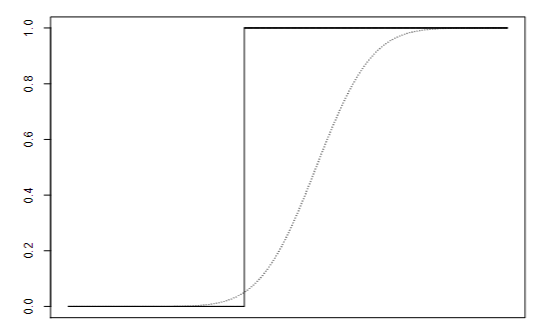
\includegraphics{figures/power_fuction.png}
    \caption[]{效应函数}
\end{figure}

然而这一般只出现在某些很简单的情况(例如$\Uniform(0,1) \vs \Uniform(2,3)$)才有可能发生。通常情况是如果要降低 $\alpha$,则需要扩大接受域的范围,而这会减小拒绝域的范围,导致 $\beta$ 增大;如果要减小 $\beta$,则需要扩大拒绝域的范围,而这会减小接受域的范围,导致 $\alpha$ 增大。

Neyman-Pearson范式将原假设与对立假设置于不平等的地位:显著性水平$\alpha$将被优先考虑,保证其低于某个固定值(例如0.1,0.05或0.01),这称之为保护原假设;接下来再尝试构造一个效应函数 $\pi(\theta;W),\ \theta \in \Theta_A$尽量小的检验。这称之为(显著性) $\alpha$级别的检验。

在显著性为 $\alpha$的前提下,什么是最好的检验?如何比较两个检验哪个更好?

\begin{definition}[一致最大功效检验]
    若在所有显著性为 $\alpha$的检验中,存在一种检验,在任意 $\theta \in \Theta_A$中,其效应函数都大于等于其他检验,则称这种检验为\textbf{一致最大功效检验}(uniformly most powerful tests, UMP)。
\end{definition}

\subsection{p值}

继续考虑例题\ref{ex:coins}的情景。$X \sim \Binomial(10, p)$,
\[ H_0: p=0.5 \vs H_A : p = 0.7 \]
在这种情况中,观测值$X$越大,对 $H_A$的支持越强,即拒绝域应包含$X$中的较大值。能够越强力地支持$H_A$的观测值称\textbf{越极端}的。若将拒绝域设为 $W=\{ 7,8,9,10 \}$,则显著性水平为
\[ \alpha = \P(X \in W|p=0.5) = 0.18 \]
效应为
\[ 1-\beta= \P(X \in W|p=0.7)=0.65\]

\begin{definition}
    
\end{definition}

\subsection{统计显著性}

\section{一些标准检验}

\section{然似比检验}

\begin{definition}[似然比]
    设样本 $x=(X_1,\cdots X_n)$的联合概率密度(质量)函数为 $f \in \Theta=\{ f_0, f_A \}$,检验为:
    \[ H_0: f = f_0 \vs H_A: f=f_A \]
    则称下式为检验\textbf{似然比}(likehood ratio)。
    \[ \frac{f_0(x)}{f_A(x)} \]
\end{definition}

这也是体现数据极端性的一种定义,当似然比越小,则数据越极端。为何不用 $f_0(x)-f_A(x)$体现?$f_0(x), f_A(x)$往往很小,即使两者比例差很大时,其差值也很小,不能体现其意义。

\begin{theorem}[Neyman-Pearson 引理]

\end{theorem}


\begin{problemset}[错题记录]
    \item (茆7.1.1)
    \item
\end{problemset}
